\documentclass{article} %选择文档类型,我们如果是做期末大作业的话选article就可以了
\usepackage{anyfontsize}
%正如c++需要import库来实现各种各样的功能,Latex也需要调用宏包来实现各种各样的功能
\usepackage{amsmath}  %调用公式宏包
\usepackage{graphicx} %调用插图宏包
\graphicspath{{code_Latex/}}
\usepackage{ctex}     %调用中文宏包
\usepackage{float}
\usepackage{cite}


%\begin{document}这句话之前是导言区,这句话以后就开始写正文了
%可以把导言区理解为int main()函数之前的内容,而正文就是int main()主函数的部分了
\usepackage{geometry}
\geometry{left=1.5cm,right=0.5cm,top=1.0cm,bottom=1.5cm}

\begin{document}
    \title{\centerline{数逻实验一报告}}
    \date{大二秋 实验一:寄存器}
    \author{信息学部计算机与电子通信7班 2023311704 王昕远 t2 612}
    \maketitle
    \thispagestyle{empty}


\section{寄存器}
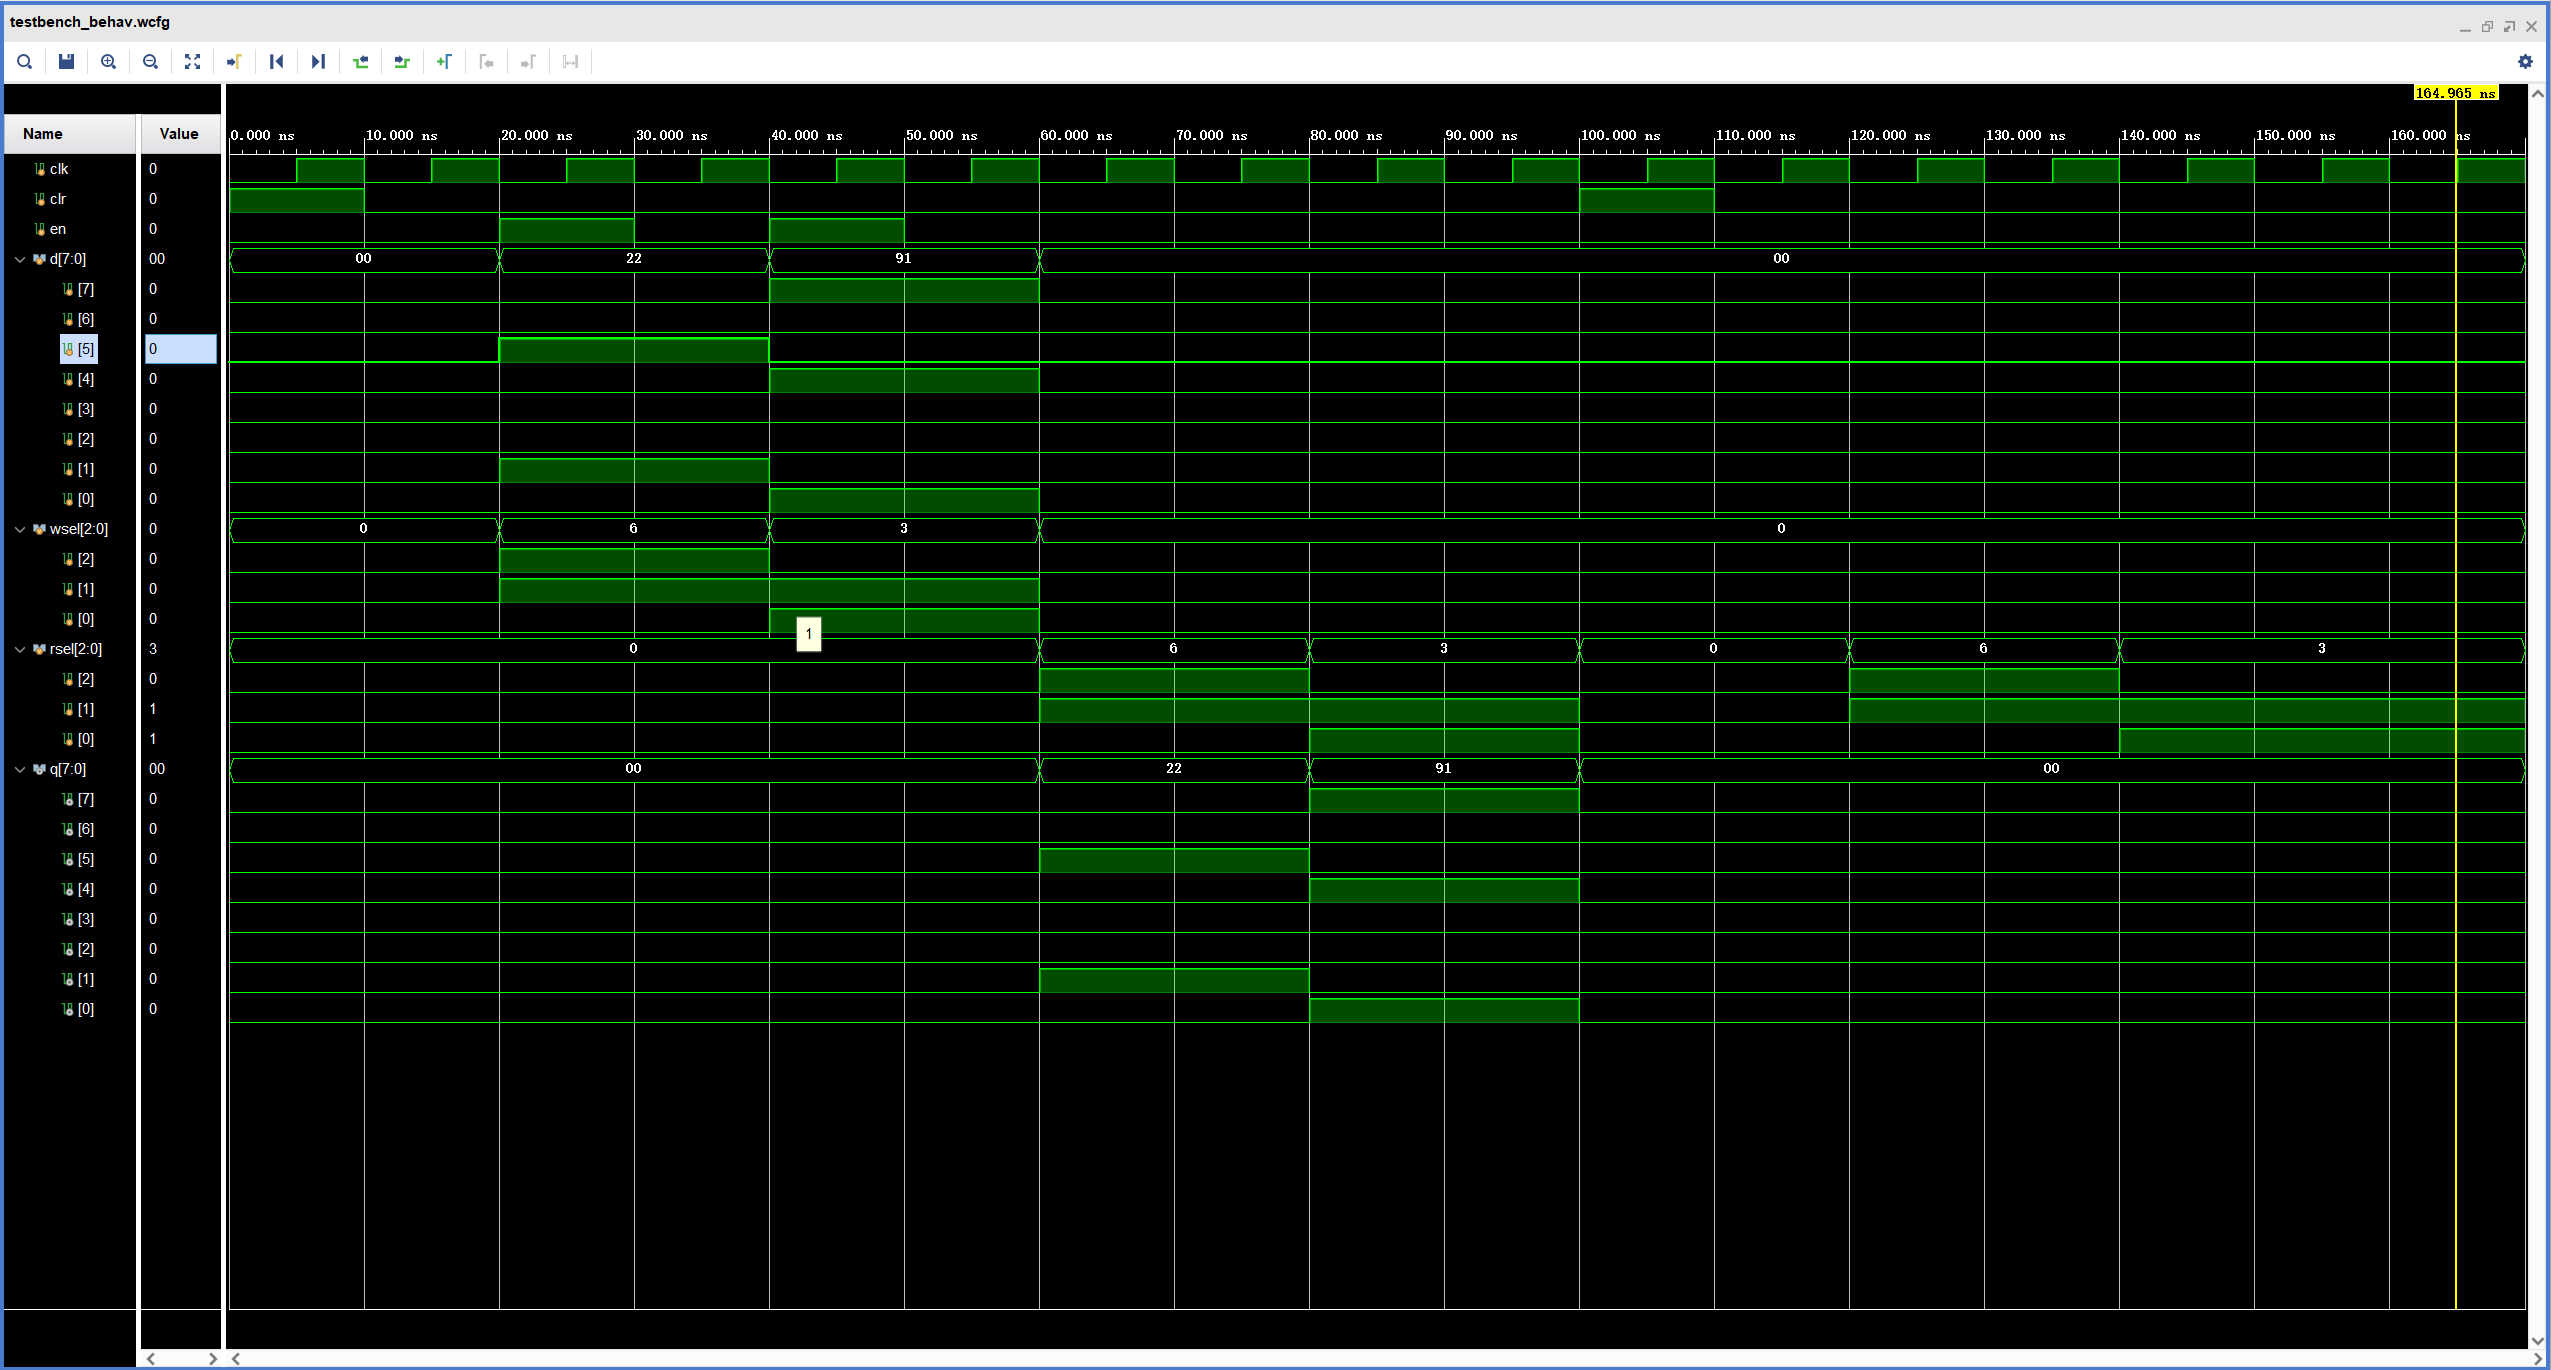
\includegraphics[width=0.8\textwidth]{1.png}\par
信号说明:复位信号 clr 、使能 en 、数据 d 为输入,q 为输出\par
从波形可以看出:\par

(1)寄存器初始复位:0-10ns,clr为1处于复位态,输出q一直为0。\par

(2)寄存器110写入:20ns-30ns,clr为0,en为1,输入d变为00100010,在时钟上升沿到来的时候存储;\par
(3)寄存器011写入:40ns-50ns,clr为0,en为1,输入d变为10010001,在时钟上升沿到来的时候存储;\par

(4)寄存器110读取:60ns-80ns,clr为0,d变为0,输出q读出寄存器中存储的值00100010;\par
(5)寄存器011读取:80ns-100ns,clr为0,d变为0,输出q读出寄存器中存储的值10010001;\par
(6)寄存器异步清零:100ns-110ns,clr为1,寄存器储存的数据在复位clr变为1的同时立刻变为0,异步清零。\par

(7)寄存器110读取:120ns-140ns,clr为0,输出q读出寄存器中存储的值00000000;\par
(8)寄存器011读取:140ns-160ns,clr为0,输出q读出寄存器中存储的值00000000;\par



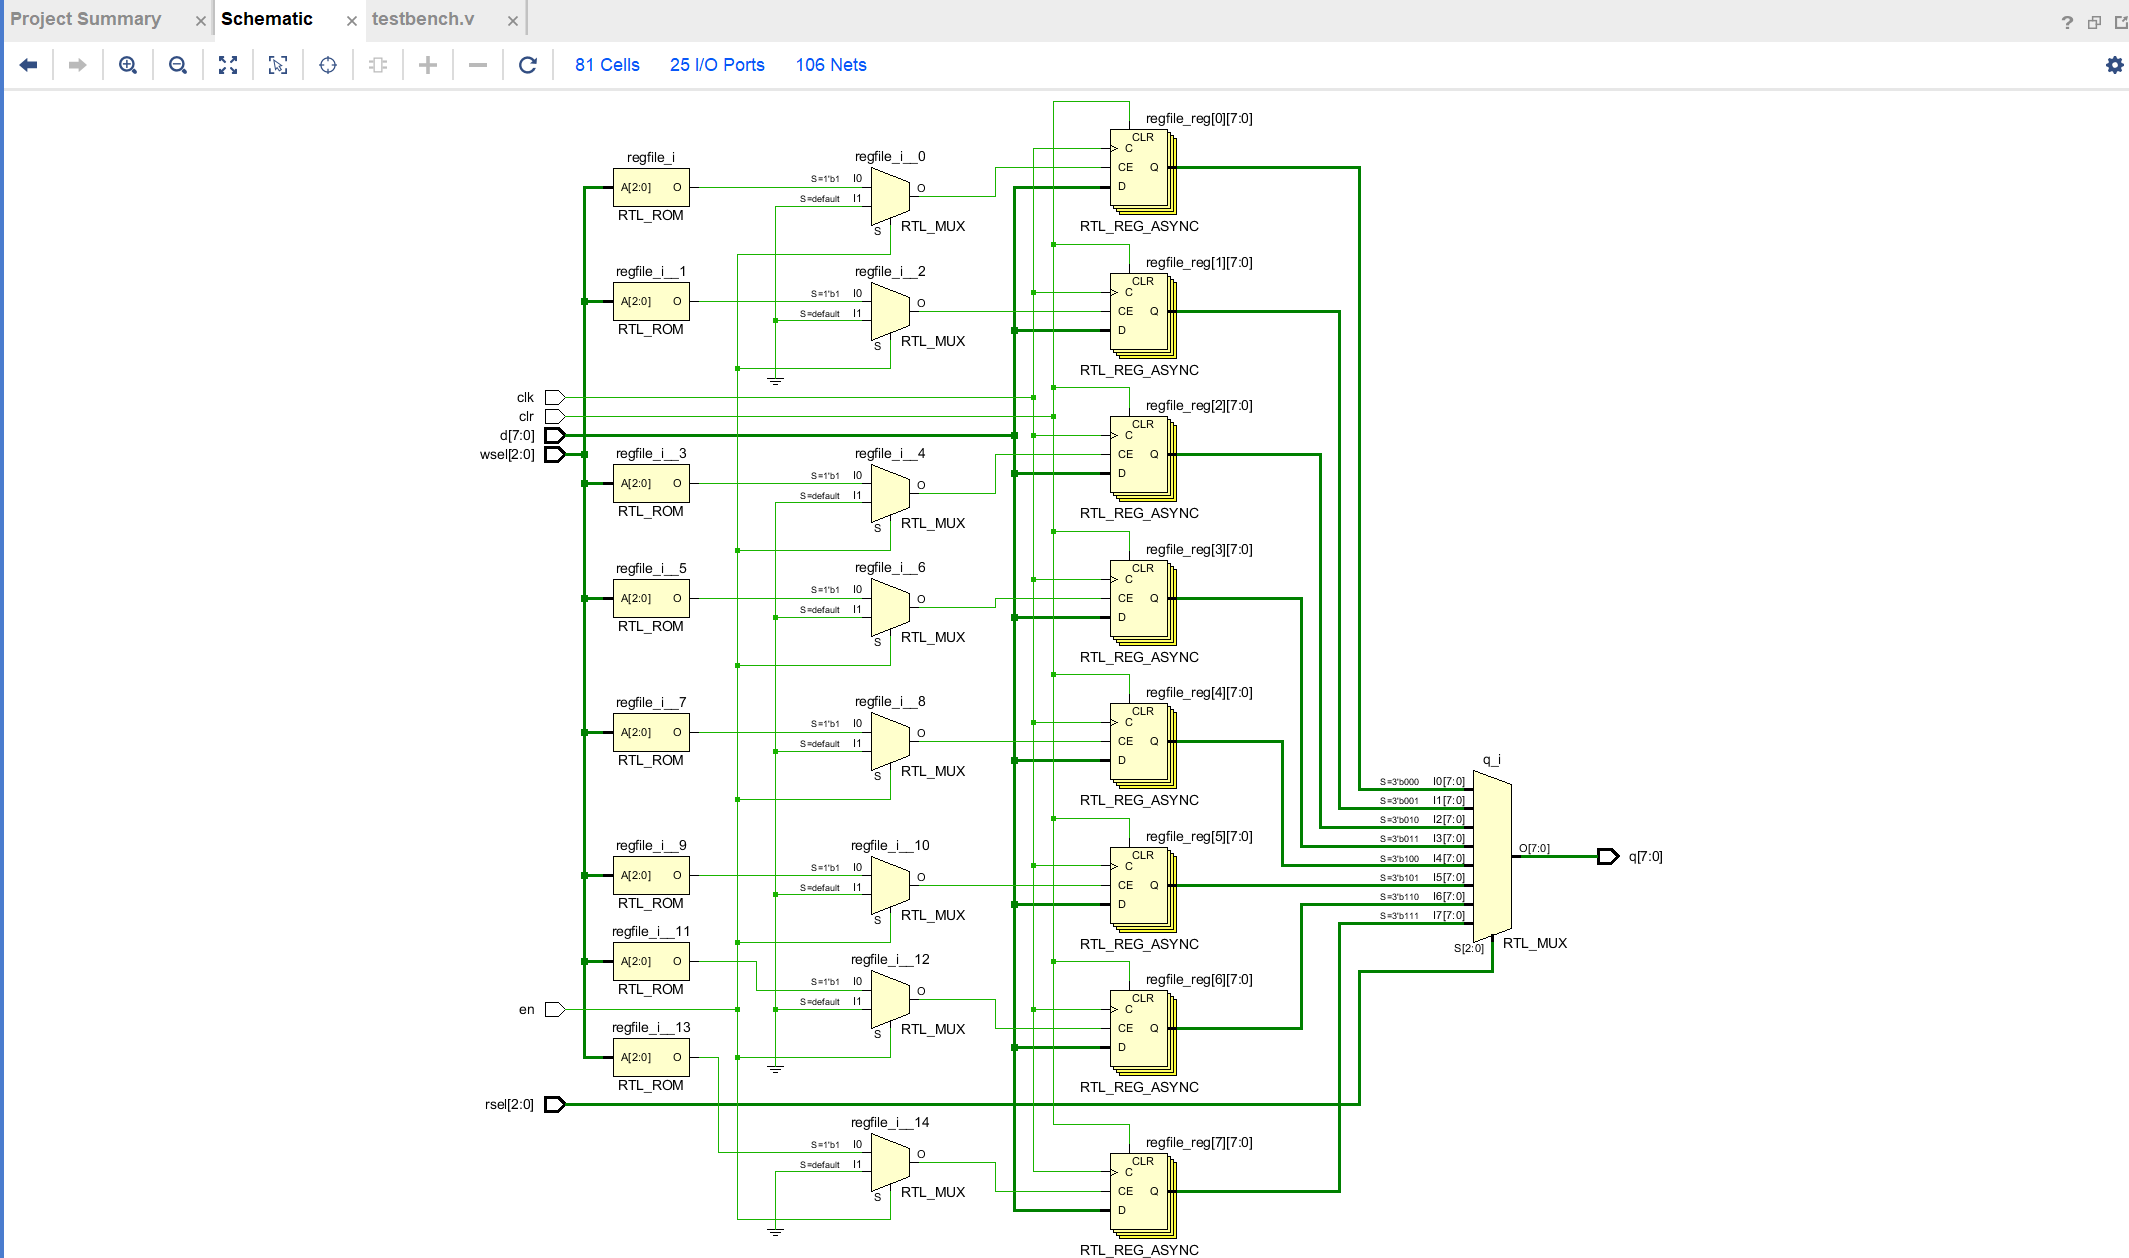
\includegraphics[width=0.8\textwidth]{2.png}\par
RTL Analysis\par
\par

$$
$$
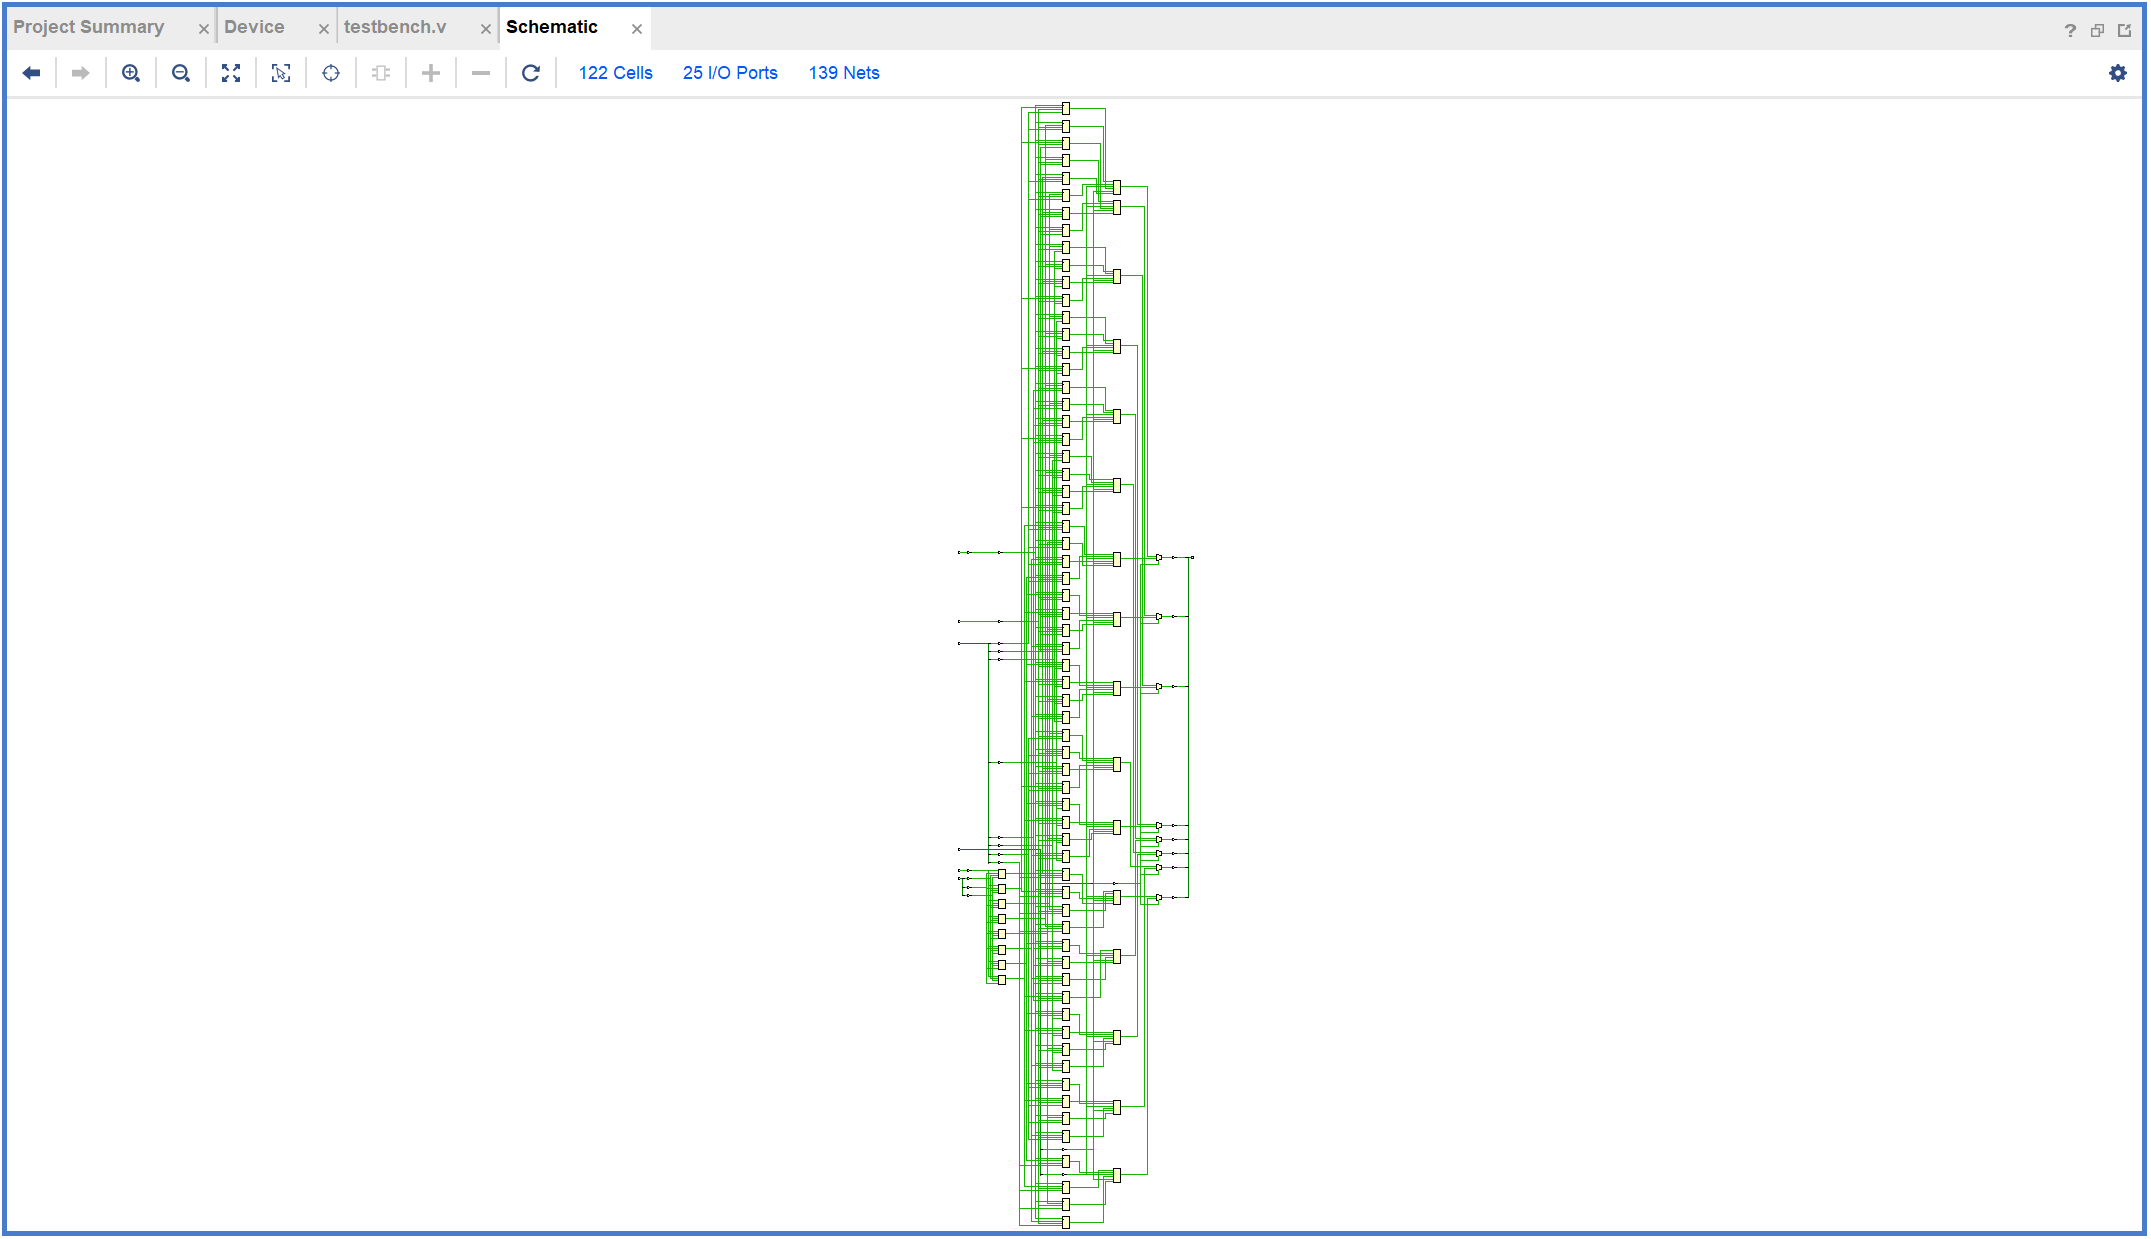
\includegraphics[width=0.8\textwidth]{3.png}\par
Synthesis schematic\par


\section{阻塞}
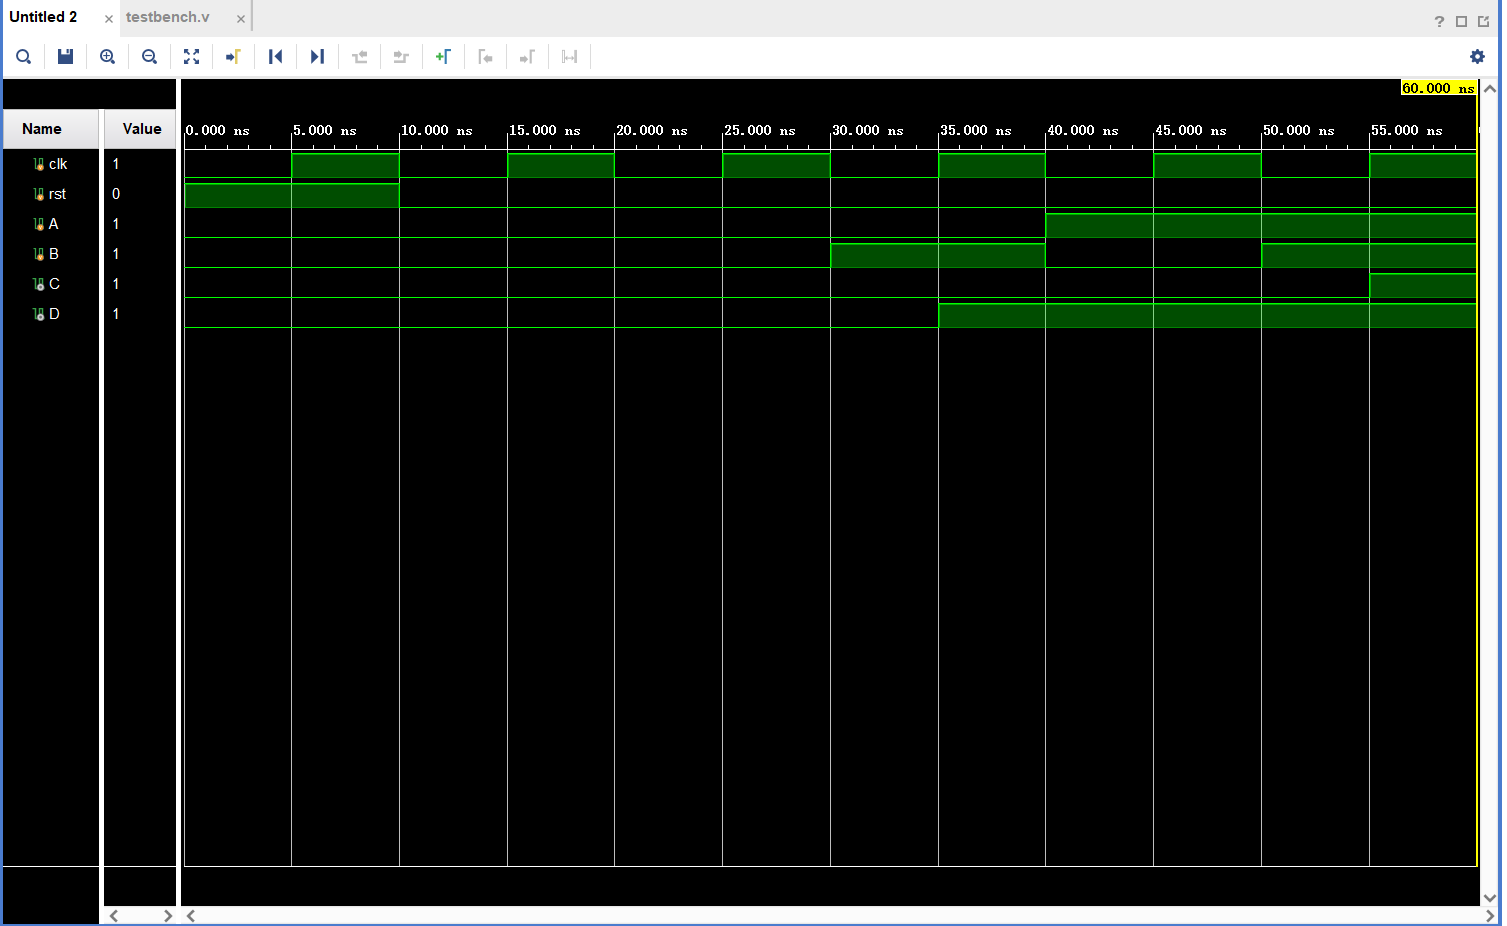
\includegraphics[width=0.8\textwidth]{11.png}\par
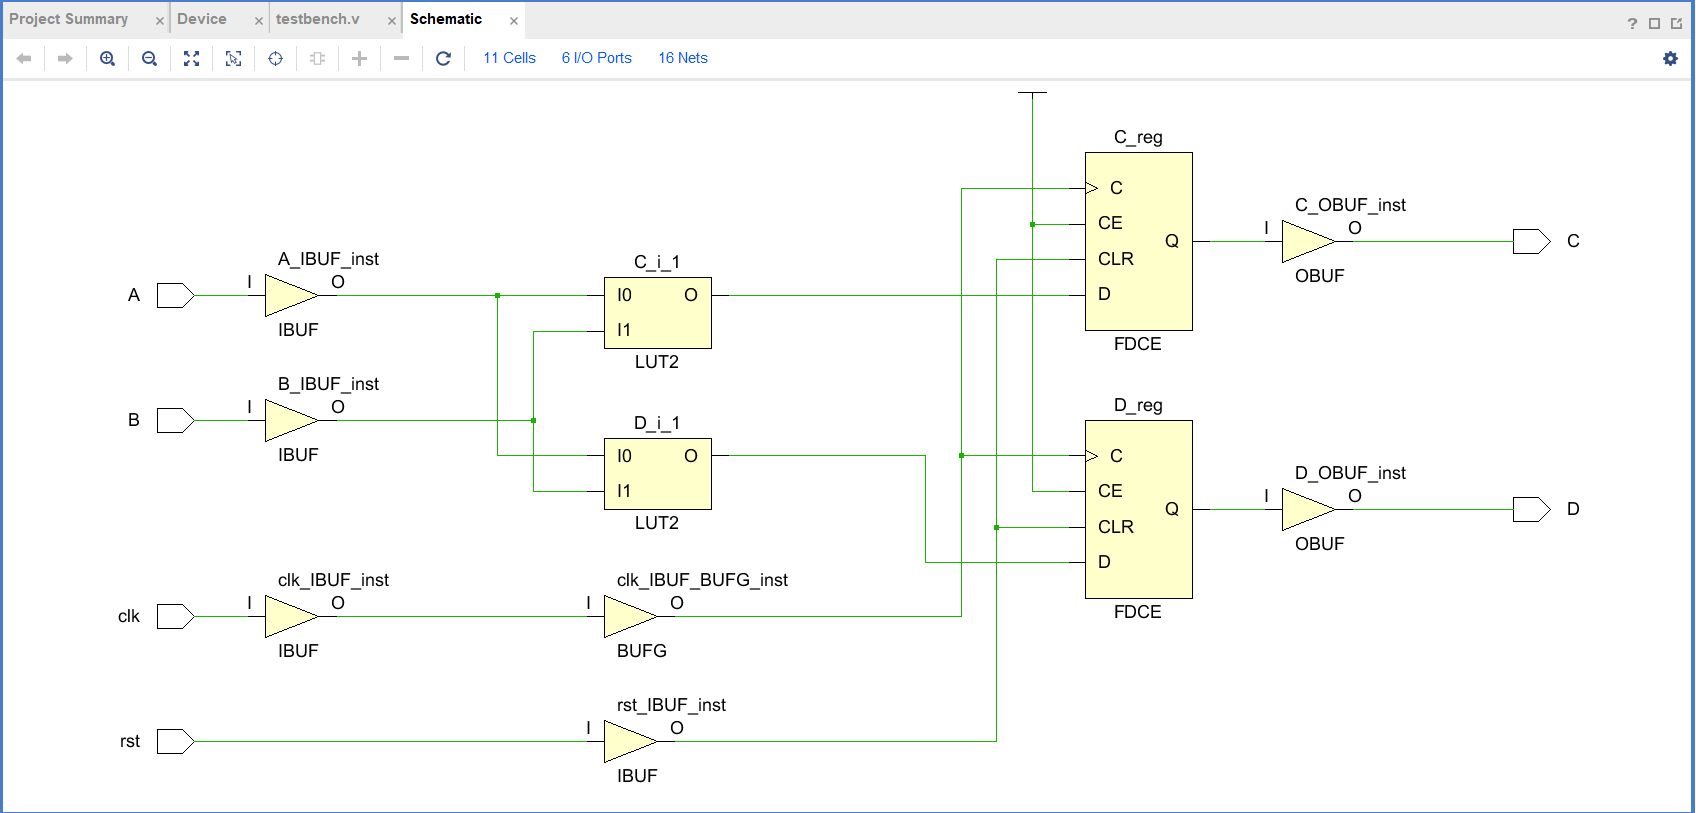
\includegraphics[width=0.8\textwidth]{12.png}\par
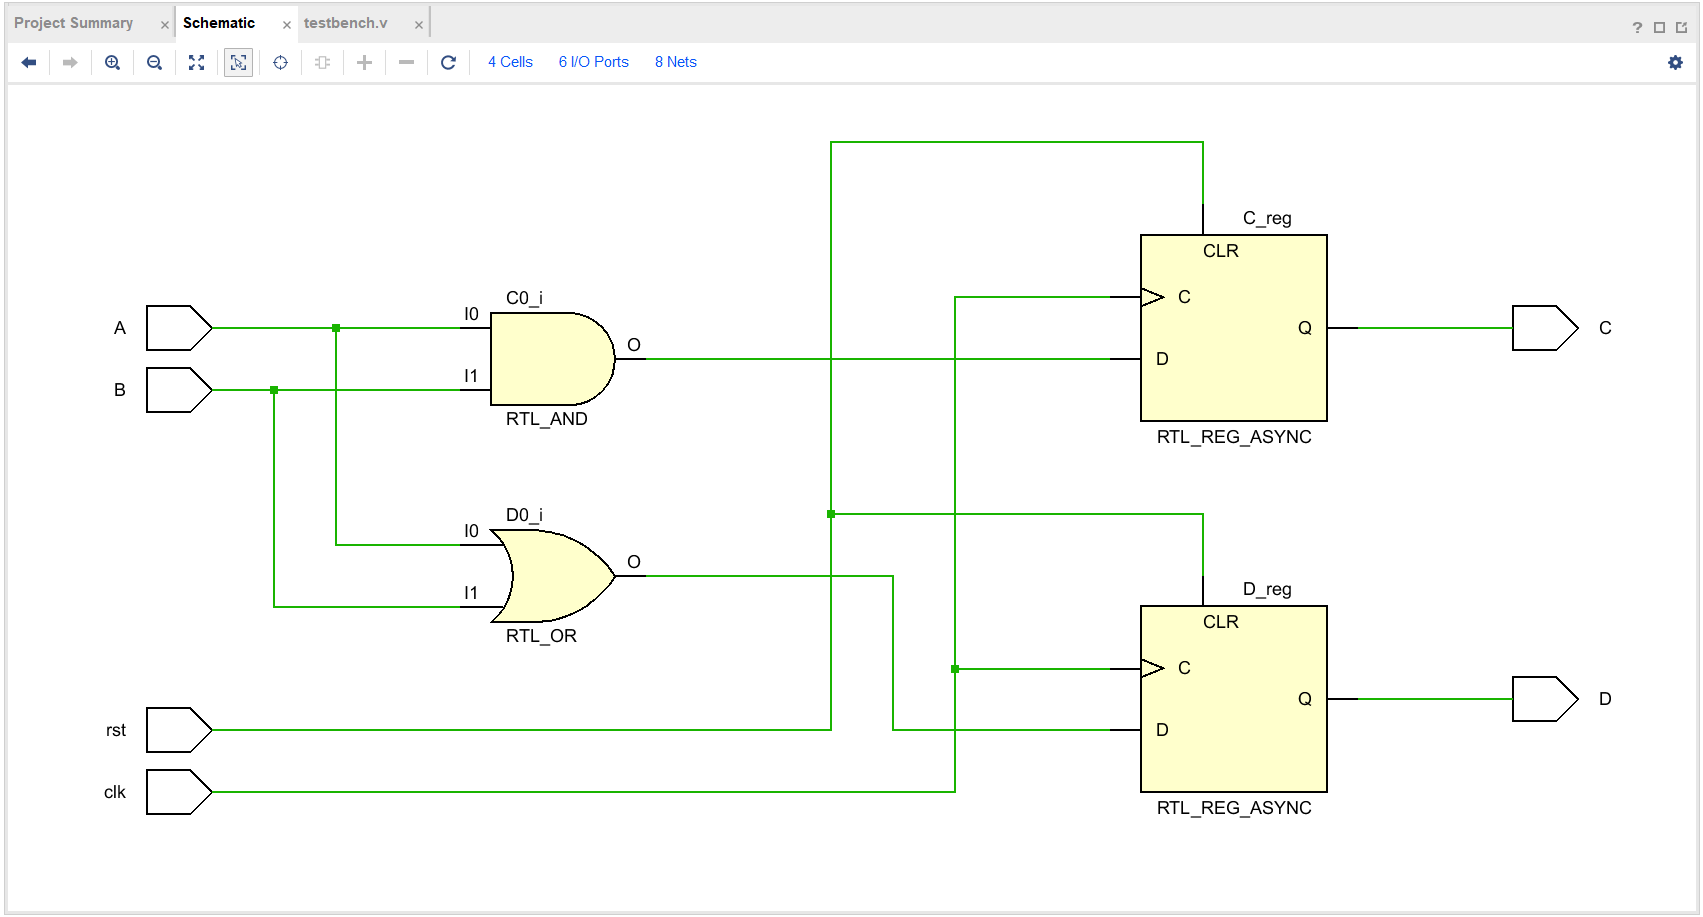
\includegraphics[width=0.8\textwidth]{13.png}\par
\section{无阻塞}
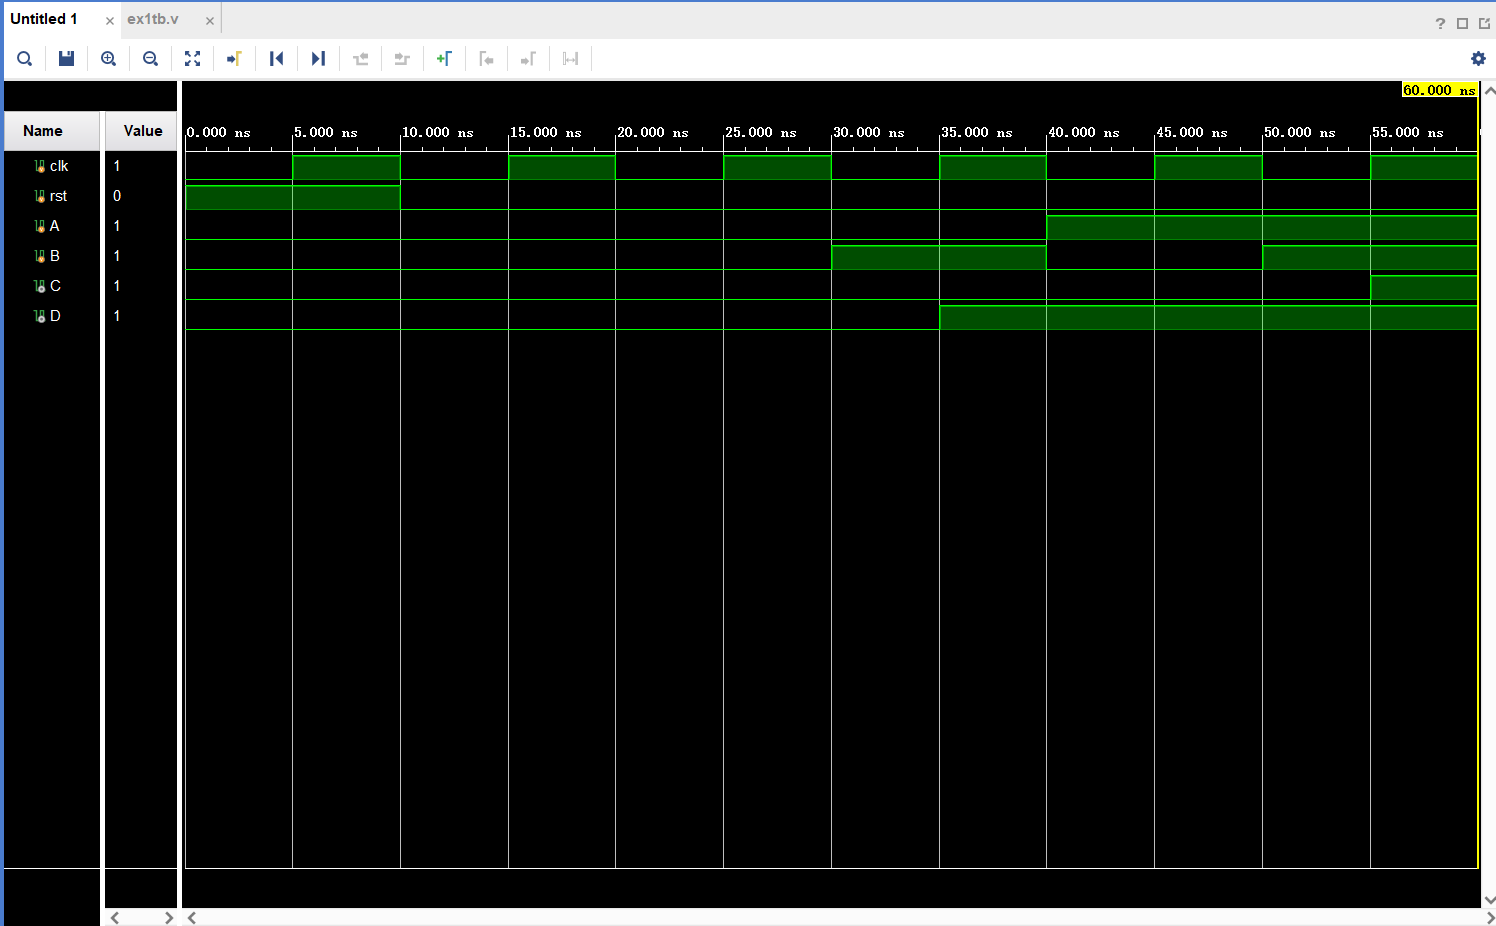
\includegraphics[width=0.8\textwidth]{21.png}\par
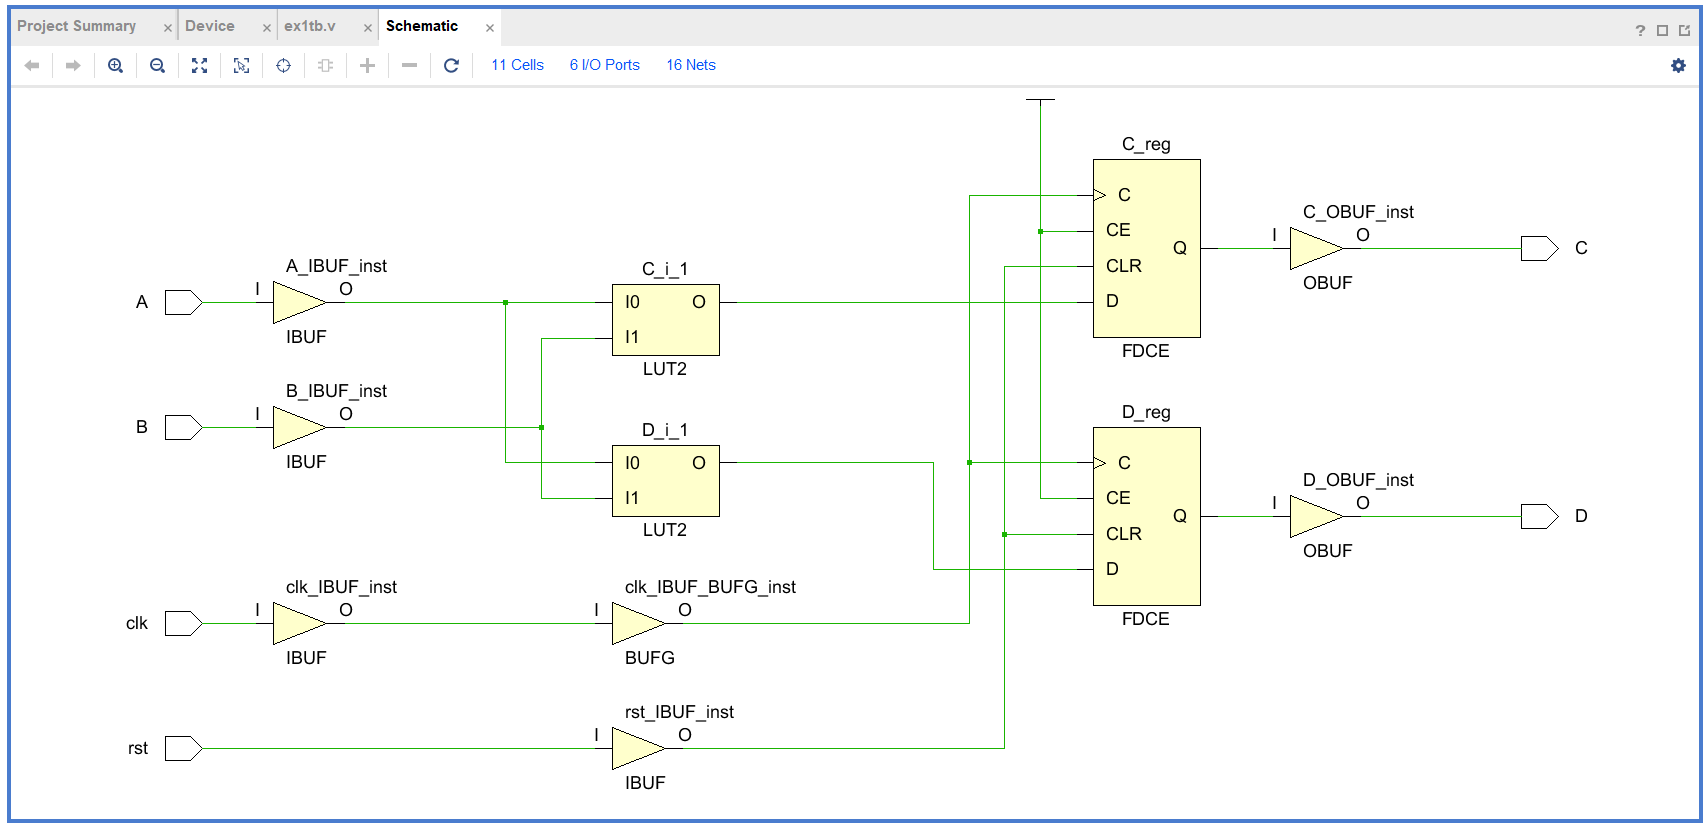
\includegraphics[width=0.8\textwidth]{22.png}\par
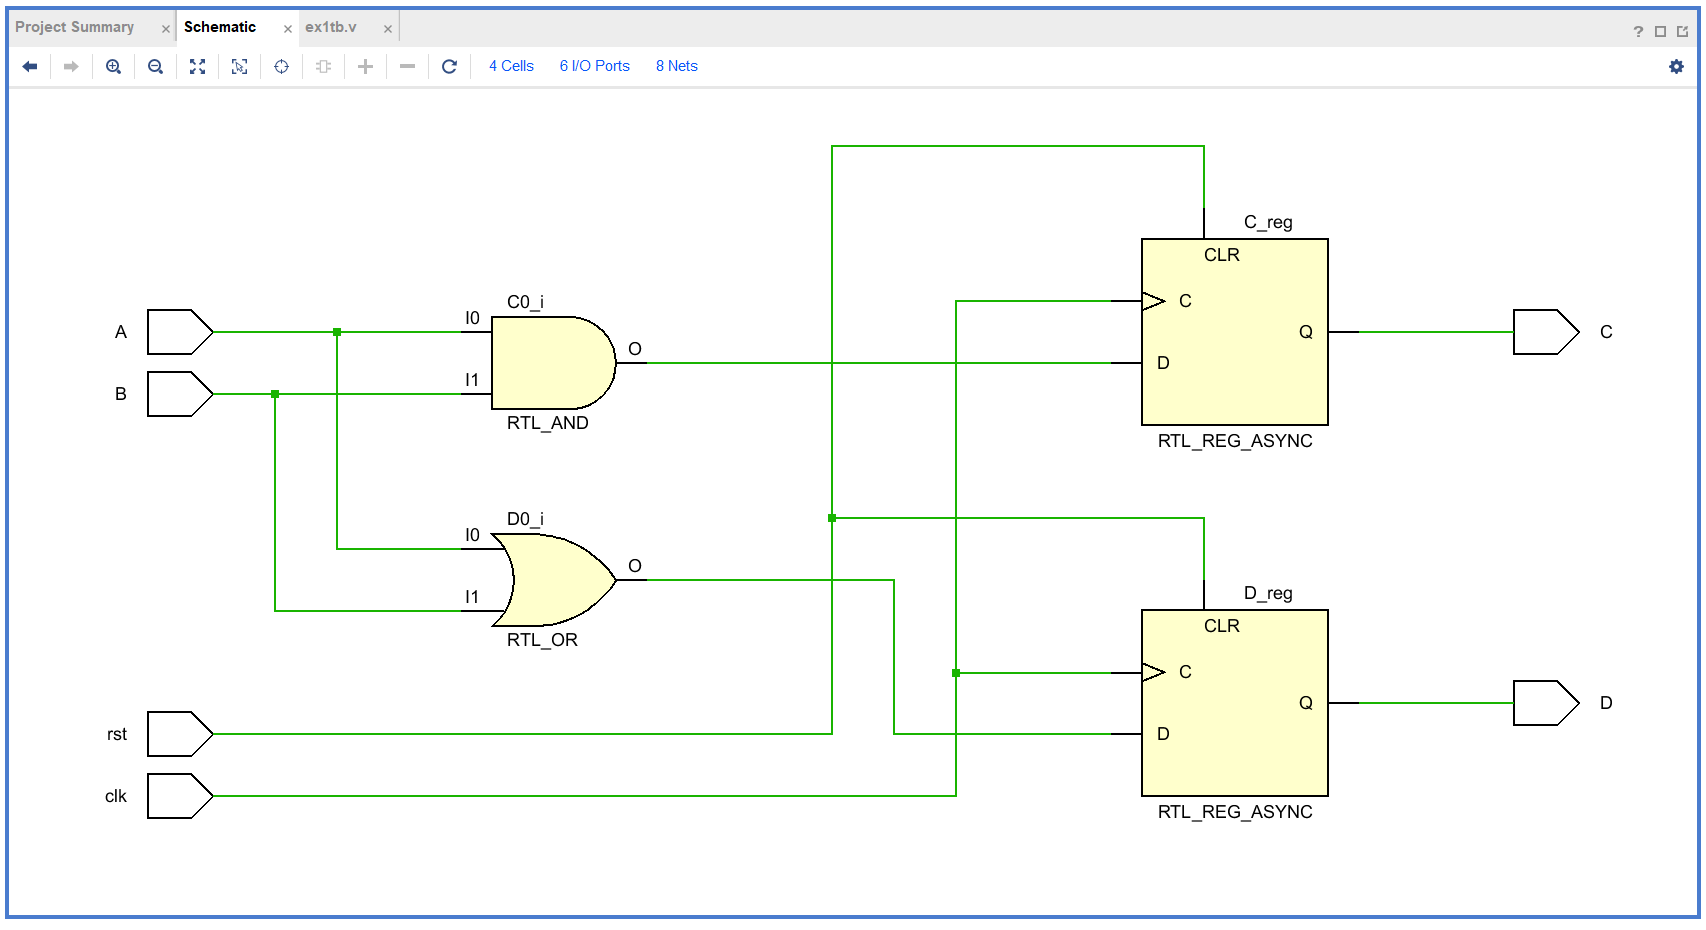
\includegraphics[width=0.8\textwidth]{23.png}\par
\section{分析}
阻塞赋值适合在组合逻辑中使用,因为它按照顺序执行,然后理解与调试。\par
非阻塞赋值适合在时序逻辑中使用,因为它更符合硬件中的硬件更新行为,避免产生不期望的时序问题。\par
在该实验中的三张图并未体现出差异.

$$
$$









\end{document}